\documentclass[12pt, letterpaper]{article}
\usepackage{graphicx} % Required for inserting images
\usepackage{hyperref}
\usepackage{listings}
\usepackage{amssymb}
\usepackage{amsmath}
\usepackage[english]{babel}
\usepackage{nicefrac, xfrac}
\usepackage{mathtools}
\newcommand{\acc}{\\\hphantom{}\\}
\usepackage[table,xcdraw]{xcolor}
\usepackage[paper=a4paper,left=20mm,right=20mm,bottom=25mm,top=25mm]{geometry}
\renewcommand{\labelenumii}{\arabic{enumi}.\arabic{enumii}}
    \renewcommand{\labelenumiii}{\arabic{enumi}.\arabic{enumii}.\arabic{enumiii}}
    \renewcommand{\labelenumiv}{\arabic{enumi}.\arabic{enumii}.\arabic{enumiii}.\arabic{enumiv}}
\title{Esercitazioni Universitarie 1 (gruppo 42)}
% \author{ Giacomo Biribicchi \and Marco Casu \and Christian Di Manno \and Alessandro Gautieri }
\date{}


\begin{document}

\maketitle


\section{Requisiti}
I dati di interesse per il sistema sono \underline{Insegnamenti} ed \underline{Esercitazioni}.
\begin{enumerate}
    \item \textbf{Insegnamento}\begin{enumerate}
        \item nome 
        \item crediti formativi
        \item docenti che lo erogano
        \item anno accademico
        \item esercitazioni dell'insegnamento
    \end{enumerate}
    \item \textbf{Docente}\begin{enumerate}
        \item nome 
        \item cognome 
        \item matricola
    \end{enumerate}
    \item\textbf{Esercitazione}\begin{enumerate}
        \item data
        \item esercizi coinvolti
    \end{enumerate}
    \item \textbf{Esercizio}\begin{enumerate}
        \item testo 
        \item soluzione 
        \item se presentato oppure risolto in aula (con soluzione)
    \end{enumerate}
    \item \textbf{Soluzione}\begin{enumerate}
        \item testo della soluzione e risultato
    \end{enumerate}
\end{enumerate}
\newpage
\section{Considerazioni}

\section{Documenti di Specifica}
\subsection{Tipi di Dato}
Matricola = Stringa [0-9]\{7\}\acc 
Anno = ("19" or "20") concat ["00","99"]\{1\}
\section{UML}
\begin{center}
    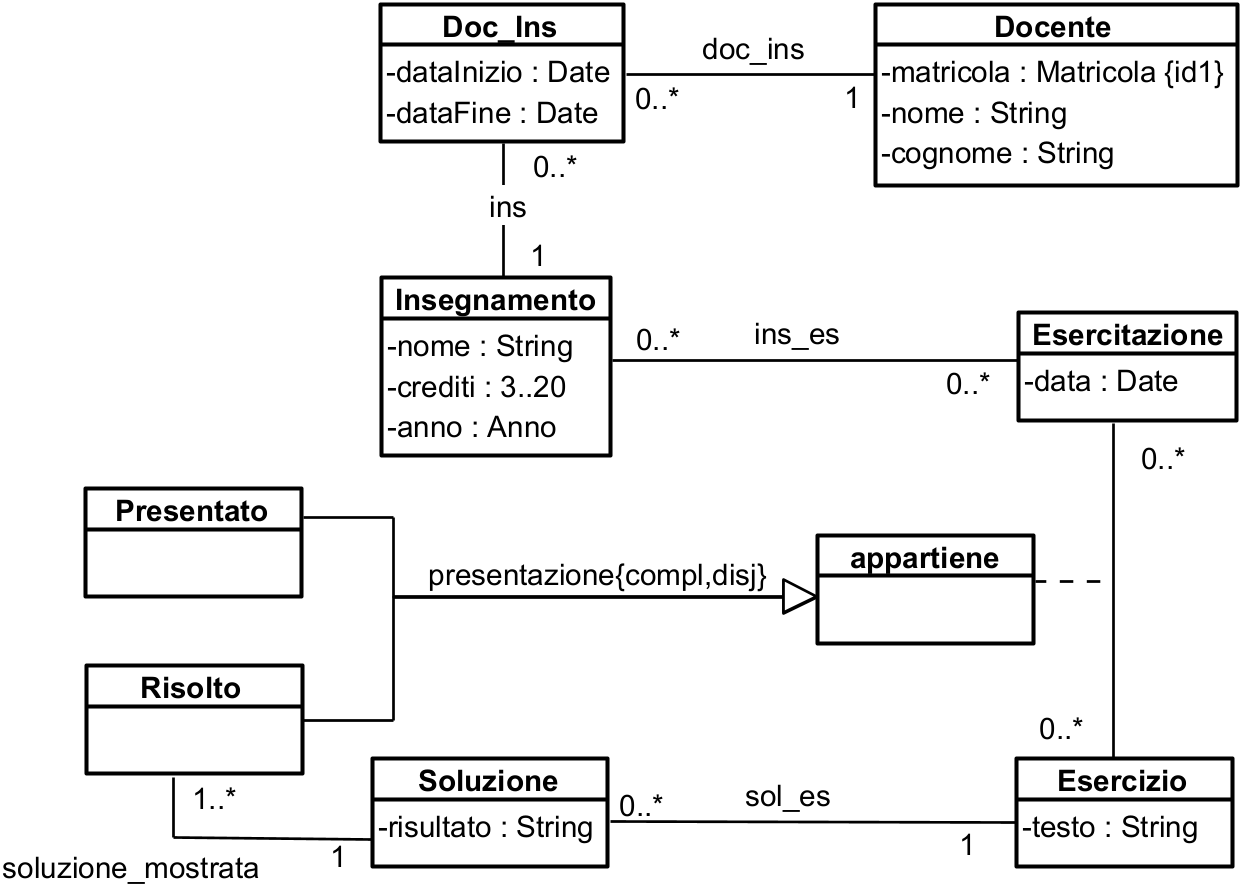
\includegraphics[width=\textwidth]{images/UML.png}
\end{center}



\end{document}

